\let\negmedspace\undefined
\let\negthickspace\undefined
\documentclass{article}
\usepackage{cite}
\usepackage{amsmath,amssymb,amsfonts,amsthm}
\usepackage{algorithmic}
\usepackage{graphicx}
\usepackage{textcomp}
\usepackage{xcolor}
\usepackage{txfonts}
\usepackage{listings}
\usepackage{enumitem}
\usepackage{tfrupee}
\usepackage{mathtools}
\usepackage{gensymb}
\usepackage[breaklinks=true]{hyperref}
\usepackage{tkz-euclide} % loads  TikZ and tkz-base
\usepackage{listings}
\usepackage{gvv}
%
%\usepackage{setspace}
%\usepackage{gensymb}
%\doublespacing
%\singlespacing

%\usepackage{graphicx}
%\usepackage{amssymb}
%\usepackage{relsize}
%\usepackage[cmex10]{amsmath}
%\usepackage{amsthm}
%\interdisplaylinepenalty=2500
%\savesymbol{iint}
%\usepackage{txfonts}
%\restoresymbol{TXF}{iint}
%\usepackage{wasysym}
%\usepackage{amsthm}
%\usepackage{iithtlc}
%\usepackage{mathrsfs}
%\usepackage{txfonts}
%\usepackage{stfloats}
%\usepackage{bm}
%\usepackage{cite}
%\usepackage{cases}
%\usepackage{subfig}
%\usepackage{xtab}
%\usepackage{longtable}
%\usepackage{multirow}
%\usepackage{algorithm}
%\usepackage{algpseudocode}
%\usepackage{enumitem}
%\usepackage{mathtools}
%\usepackage{tikz}
%\usepackage{circuitikz}
%\usepackage{verbatim}
%\usepackage{tfrupee}
%\usepackage{stmaryrd}
%\usetkzobj{all}
%    \usepackage{color}                                   >
%    \usepackage{array}                                   >
%    \usepackage{longtable}                               >
%    \usepackage{calc}                                    >
%    \usepackage{multirow}                                >
%    \usepackage{hhline}                                  >
%    \usepackage{ifthen}                                  >
  %optionally (for landscape tables embedded in another do>
%    \usepackage{lscape}
%\usepackage{multicol}
%\usepackage{chngcntr}
%\usepackage{enumerate}

%\usepackage{wasysym}
%\documentclass[conference]{IEEEtran}
%\IEEEoverridecommandlockouts
% The preceding line is only needed to identify funding in>

\newtheorem{theorem}{Theorem}[section]
\newtheorem{problem}{Problem}
\newtheorem{proposition}{Proposition}[section]
\newtheorem{lemma}{Lemma}[section]
\newtheorem{corollary}[theorem]{Corollary}
\newtheorem{example}{Example}[section]
\newtheorem{definition}[problem]{Definition}
%\newtheorem{thm}{Theorem}[section]
%\newtheorem{defn}[thm]{Definition}
%\newtheorem{algorithm}{Algorithm}[section]
%\newtheorem{cor}{Corollary}
\newcommand{\BEQA}{\begin{eqnarray}}
\newcommand{\EEQA}{\end{eqnarray}}
%\newcommand{\define}{\stackrel{\triangle}{=}}
\theoremstyle{remark}
\newtheorem{rem}{Remark}

%\bibliographystyle{ieeetr}
\begin{document}
\title{Latex Assignment1}
\author{APARNA ANAND}
\date{29 August,2023}
\maketitle
\section*{Example:-1-25 (11.10)}
\begin{enumerate}
\item Find the slope of lines:
\begin{enumerate}
\item  Passing through the points $(3,-2)$ and $(-1,4)$
\item  Passing through the points $(3,-2)$ and $(7,-2)$
\item  passing through the points $(3,-2)$ and $(3,4)$	
\item  Making inclination of $60\degree$ with the positive direction of x-axis.
\end{enumerate}
\item If the angle between two lines is $\frac{\pi}{4}$ and slope of one of the lines is $\frac{1}{2}$, find the slope of the other line.
\item Line through the points $(-2,6)$ and $(4,8)$ is perpendicular to the line through the points $(8,12)$ and $(x,24)$. Find the value of x.
\item Three points $(h,k), Q(x_1,y_1)$ and $R(x_2,y_2)$ lie on a line. Show that $(h-x_1)(y_2-y_1)=(k-y_1)(x_2-x_1)$.
\item In \figref{fig:10.9}, time and distance graph of a linear motion is given. Two positions of line and distance are recorded as, when $T=0,D=2$ and when $T=3,D=8$. Use the concept of slope, find law of motion i.e, how distance depends upon time.
\begin{figure}[h]
\centering
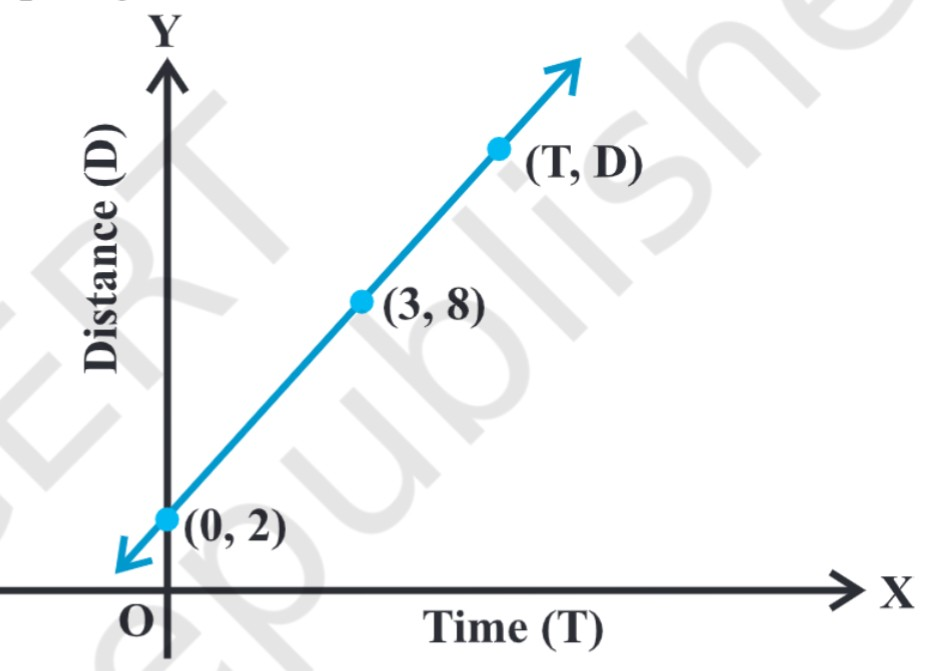
\includegraphics[width=\columnwidth]{figs/10.9.png}
\caption{10.9}
  \label{fig:10.9}
\end{figure}
\item Find the equations of the lines parallel to axes and passing through $(2,3)$.
\item Find the equation of the line through $(-2,3)$ with slope $-4$
\item Write the equation of the line through the points $(1,-1)$ and $(3,5)$.
\item Write the equation of the lines for which $\tan \theta=\frac{1}{2}$, where $\theta$ is the inclination of the line and
\begin{enumerate}[label=(\roman*)]
\item  y-intercepts is $\frac{-3}{2}$ 
\item  x-intercept is $4$.
\end{enumerate}
\item Find the equation of the lines which makes intercepts $-3$ and $2$ on the x- and y-axes respectively.
\item Find the equation of the line whose perpendicular distance from the origin is $4$ units and the angle which the normal makes with positive direction of x-axis is $15\degree$.
\item The Fahrenheit temperature $F$ and  absolute temperature $K$ satisfy a linear equation. Given that $K=273$ when $F=32$ and that $K=373$ when $F=212$. Express $K$ in terms of $F$ and find the value of $F$, when $K=0$.
\item Equation of a line is $3x-4y+10=0$, Find its
\begin{enumerate}[label=(\roman*)]
\item  Slope
\item  x and y-intercepts.
\end{enumerate}
\item Reduce the equation $\sqrt3x+y-8=0$ into normal form.Find the values of p and $\omega$.
\item Find the angle between the lines $y-\sqrt 3x-5=0$ and $\sqrt 3y-x+6=0$.
\item Show that two lines $a_1x+b_1y+c_1=0$ and $a_2x+b_2y+c_2=0$ where $b_1b-2\neq 0$ are:
\begin{enumerate}
\item parallel if $\frac{a_1}{b_1}=\frac{a_2}{b_2}$ and 
\item Perpendicular if $a_1a_2-b_1b_2=0$.
\end {enumerate}
\item Find the equation of a line perpendicular to the line $x+2y+3=0$ and passing through the point $(1,-2)$.
\item Find the distance of the point $(3,-5)$ from theline $3x-4y-26=0$.
\item Find the distaance between the parallel lines $3x-4y+7=0$ and $3x-4y+5=0$.
\item If the lines $2x+y-3=0, 5x+ky-3=0$ and $3x-y-2=0$ are concurrent, find the value of k.
\item Find the distance of the line $4x-y-0$ from the point $p(4,1)$ measured along the line making an angle of $135\degree$ with the positive x-axis.
\item Assuming that straight lines work as the plane mirror for a point, find the image of the point $(1,2)$ in the line $x-3y+4=0$.
\item Show that the area of the triangle formed by the lines $y=m_1x+c_1, y=m_2x+c_2$ and $x=0$ is $\frac{c_1-c_2^2}{2|m_1-m_2|}$
\item A line is such that its segment between the lines $5x-y+4=0$ and $3x+4y-4=0$ is bisected at the point $(1,5)$. Obtain its equation.
\item Show that the path of a moving point such that its distances from two lines $3x-2y=5$ and $3x+2y=5$ are equal is a straight line.
\end{enumerate}
\end{document}
 
